\chapter{Introduzione}
\textbf{Crittologia}: l'arte delle scritture segrete, può essere divisa in 3 macro argomenti:
\begin{enumerate}[nosep]
    \item \textbf{crittografia}: come \textit{trasformare} messaggi per proteggerne il contenuto (l'informazione).
    \item \textbf{steganografia}: come \textit{nascondere} messaggi per evitare che venga individuato (ex. \textbf{least significant bit steganography}).
    \item \textbf{crittoanalisi}: come \textit{analizzare} messaggi e rivelarne l'informazione.   
\end{enumerate}

\section{Crittografia Classica}
La sicurezza della crittografia classica si basa unicamente sulla \textbf{segretezza} del \textbf{metodo} (noto solo al \textit{sender} e al \textit{receiver}), considerava come una tipologia di attacco quello \textbf{passivo} (\textit{read only}). Basandosi su questi concetti il suo utilizzo in applicazioni reali è molto limitato (nel senso moderno), considerando la comunicazione in termini di scambio di informazioni in linguaggio naturale. \\
Alcuni esempi: \textbf{scytale} (\textit{transposition cipher}), \textbf{caesar cipher} (\textit{shift cipher}) e \textbf{vigenere cipher}.

\newpage
\section{Crittografia Moderna}
\subsection{Encryption only}
La crittografia moderna si basa su due principi:
\begin{enumerate}[nosep]
    \item \textbf{Kerckhoffs principles}:
    \begin{itemize}[nosep]
        \item gli algoritmi devono essere pubblici.
        \item la sicurezza del metodo si deve basare sulla \textbf{segretezza} della \textbf{chiave}.
        \item uno schema deve essere ``praticamente'', se non ``matematicamente'' indecifrabile
    \end{itemize}
    \item \textbf{Shannon principles}:
    \begin{itemize}[nosep]
        \item \textbf{confusione}: ogni bit del crittogramma deve dipendere da più bit della chiave, oscurando, però, la correlazione tra le due.
        \item \textbf{diffusione}: se viene cambiato un singolo bit del testo in chiaro, allora almeno la metà dei bit del crittogramma devono cambiare, e viceversa.
    \end{itemize}
\end{enumerate}
Nella crittografia moderna lo spazio delle chiavi deve essere sufficentemente ampio per evitare una ricerca esaustiva su di esso, in più, nessuna informazione (nè del \textit{plaintext}, né della \textit{key}) deve poter essere estrapolata dal \textit{ciphertext}. Viene detto che il \textit{ciphertext} deve essere \textbf{indistinguibile} da una sequenza di bit \textit{random}.

\subsection{Extended and applied settings}
Gli avversari (i crittoanalisti) non sono più unicamente \textbf{passivi}, ma bisogna modellare delle tipologia di avversari che siano capaci anche di \textbf{interagire} con i nostri sistemi e \textbf{manipolare} dei messaggi. \\
Per ognuna di queste modellazioni è necessario \textbf{provare la sicurezza} dei sistemi andando a \textbf{definire} delle attività (tramite la comprensione e modellare cosa è ``sicuro'') e \textbf{costruendo} attività (progettandole e provandone la veridicità). \\ \newline
Bisogna definire le \textbf{primitive}, gli \textbf{schemi}, i \textbf{protocolli} e le \textit{applicazioni} che vengono utilizzati, andandoli ad analizzare separatamente e completa. \\
$\Rightarrow$ può essere necessario costruire schemi e protocolli modellati su misura per applicazioni reali inerenti ad un certo caso d'uso: \textcolor{red}{\textbf{Applied Cryptography}}.

\newpage
\section{Crittografia Applicata}
È un layer di astrazione che può essere (quasi) direttamente mappato all'interno di una soluzione per un caso d'uso reale (quindi tecniche ``pratiche''). Siccome analizziamo \textbf{soluzioni pratiche} bisogna gestire possibili errori dovuti ad \textbf{implementazioni} o \textbf{\textit{deployment}} errati. I protcolli sicuri assumono che un attaccante tenti di accedere alle informazioni in transito (violazione della \textbf{confidenzialità}) e cerchi di impersonificare un mittente (violazione dell'\textbf{autenticazione}). \\ 
Una delle sicurezze che deve garantire un protocollo sicuro è la \textbf{confidenzialità}. \\ \newline
Quando si studi/analizza/progetta un protocollo crittografico è necessario identificare:
\begin{itemize}[nosep]
    \item \textbf{system model}: descrive lo scenario (``idealmente'') di utilizzo, andando a definire: gli attori \textbf{legittimi}, la \textbf{tipologia di protocollo} utilizzata, le \textbf{informazioni} possedute dagli attori legittimi, e altre informazioni sullo scenario applicativo.
    \begin{boxA}
        \textcolor{orange}{\textbf{Esempio}} \\
        Un protocollo sicuro che ha come \textbf{scopo} proteggere le informazioni scambiati tra due attori: \textbf{Alice} e \textbf{Bob} quando un possibile attaccante \textbf{Eve} può accedere direttamente all'informazione tramite il canale fisico. 
        \smallskip

        {\centering
            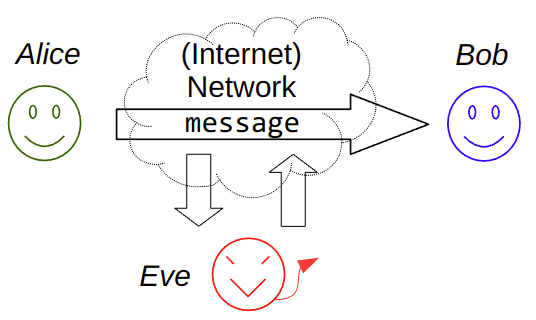
\includegraphics[width=0.3\textwidth]{img/system_model.png}
        \par}
    \end{boxA}
    \item \textbf{threat modelling} (modellazione della tipologia di attaccante): abbiamo identificato degli attori legittimi, ma quanto sono affidabili? Modelliamo il protocollo sulla base dell'attaccante.
    \begin{enumerate}[nosep]
        \item che operazioni può effettuare sui dati: solo lettura, modifica, inserimento o eliminazione dei dati.
        \item qual è la superficie di attacco e cosa può provare a fare: ha accesso ad alcune funzionalità (cifrazione/decifrazione), che tipologia conoscenza (\textit{white}/\textit{gray}/\textit{black box}), quanti tentavi si hanno: adattivo o meno.
    \end{enumerate}
    \begin{boxA}
        \textcolor{orange}{\textbf{Esempio}} \\
        Cosa può fare \textbf{Eve} per compromettere la comunicazione: leggere, manipolare le informazioni in transito, compromissione di un attore legittimo.
        \smallskip

        {\centering
            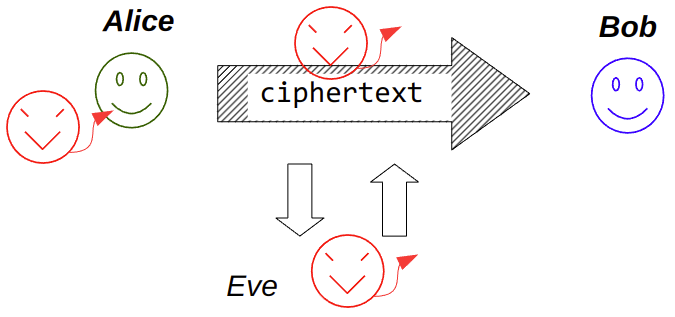
\includegraphics[width=0.3\textwidth]{img/threat_modelling.png}
        \par}
    \end{boxA}
    \item \textbf{security guarantees}: quale aspetto di sicurezza vogliamo garantire: \textbf{confidenzialità}, \textbf{integrità} (autenticazione), \textbf{disponibilità}, \textbf{non ripudio} (è anche presente il concetto di \textbf{\textit{forward security}}).
    \item \textbf{cryptogrphy settings}: le due classi principali sono: crittografia \textbf{simmetrica} (le funzioni di \textit{encrypt} e \textit{decrypt} utilizzano lo stesso \textbf{segreto}) e crittografia \textbf{asimmetrica} (sono presenti due differenti \textbf{chiavi}, uno utilizzabile durante la funzione di \textit{encrypt} - \textit{public} - e l'altro utilizzato durante la funzione di \textit{decrypt} - \textit{secret}).
    \item \textbf{security assumptions of a proposed scheme}
\end{itemize}

Alcuni \textbf{protocolli}:
\begin{enumerate}[nosep]
    \item \textbf{\textit{Secure key exchange protocol}} (scambio sicuro di chiavi): Alice e Bob non hanno nessuna \textbf{chiave}, ne vogliono ottenere una \textbf{sicura} e \textbf{condivisa} comunicando su un canale sincrono e non sicuro.
    \item \textbf{\textit{Secure storage}}
\end{enumerate}